\documentclass[tikz,border=1pt]{standalone}
\usepackage{tikz}
\usetikzlibrary{arrows,positioning,shapes,fit,calc}
\begin{document}
    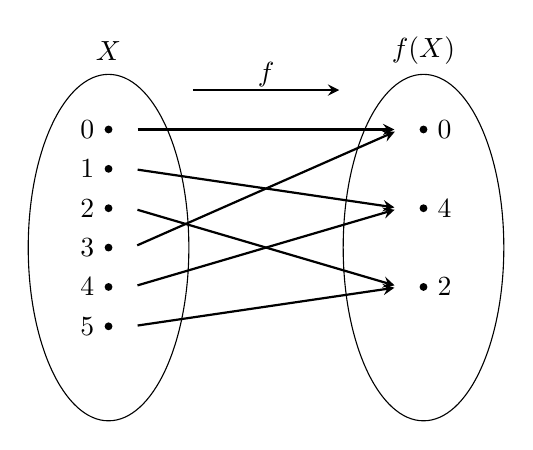
\begin{tikzpicture}[
    >=stealth,
    bullet/.style={
        fill=black,
        circle,
        minimum width=1pt,
        inner sep=1pt
    },
    projection/.style={
        ->,
        thick,
        shorten <=2pt,
        shorten >=2pt
    },
    every fit/.style={
        ellipse,
        draw,
        inner sep=0pt
    }
    ]
    \node at (2,4.7) {$f$};
    \draw[projection] (1,4.5) -- (3,4.5);
    \node at (0,5) {$X$};
    \node at (4,5) {$f(X)$};

    \node[bullet,label=left:$0$] (START0)   at (0,4){};
    \node[bullet,label=right:$0$] at (4,4){};
    \node[bullet,label=left:$1$] (START1)   at (0,3.5){};
    \node[bullet,label=left:$2$] (START2)   at (0,3){};
    \node[bullet,label=right:$4$] at (4,3){};
    \node[bullet,label=left:$3$] (START3)   at (0,2.5){};
    \node[bullet,label=left:$4$] (START4)   at (0,2){};
    \node[bullet,label=right:$2$] at (4,2){};
    \node[bullet,label=left:$5$] (START5)   at (0,1.5){};


    \draw (0,2.5) ellipse (1.02cm and 2.2cm);
    \draw (4,2.5) ellipse (1.02cm and 2.2cm);

    \draw[projection] (0.3,4) -- (3.7,4);
    \draw[projection] (0.3,3.5) -- (3.7,3);
    \draw[projection] (0.3,3) -- (3.7,2);
    \draw[projection] (0.3,2.5) -- (3.7,4);
    \draw[projection] (0.3,2) -- (3.7,3);
    \draw[projection] (0.3,1.5) -- (3.7,2);
    \end{tikzpicture}
\end{document}
